\begin{surferPage}[Barth-Sextic]{The Barth Sextic}
    This surface of degree $6$ (sextic) was constructed by Wolf Barth in 1996.
    
    The Barth Sextic has $65$ singularities altogether.
%    (wenn man die $15$ im Bild nicht sichtbaren, ``unendlich fernen'', mitz�hlt)%
   This is the maximum possible number of singularities on a sextic as shown
    shortly after Barth's construction by Jaffe and Ruberman --- so, Barth's
    world record is unbeatable!


    Barth's construction was a big surprise because for a long time people
    thought that surfaces of degree $6$ can only have $64$ singularities.

   A striking feature of the construction is its icosahedral symmetry; 
    the figure shows an icosahedron and its symmetry planes:  
%    Die Abb.\ zeigt diesen platonischen K�rper und seine Symmetrie - Ebenen: 
%    und diese Ebenen gemeinsam mit der Barth Sextik in einem Bild.     
    % 
  \begin{center}
      \vspace*{-0.1cm}
      \begin{tabular}{@{}c@{\ \ }c@{\,}c@{}}
        \begin{tabular}{@{}c}
          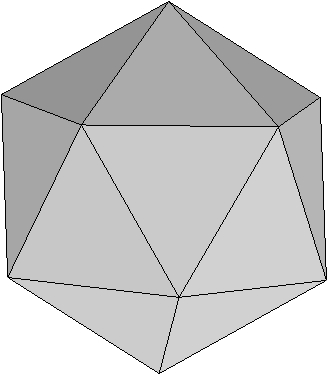
\includegraphics[width=1.4cm]{./../../common/images/icosah}
        \end{tabular}
        &
        \begin{tabular}{@{}c}
          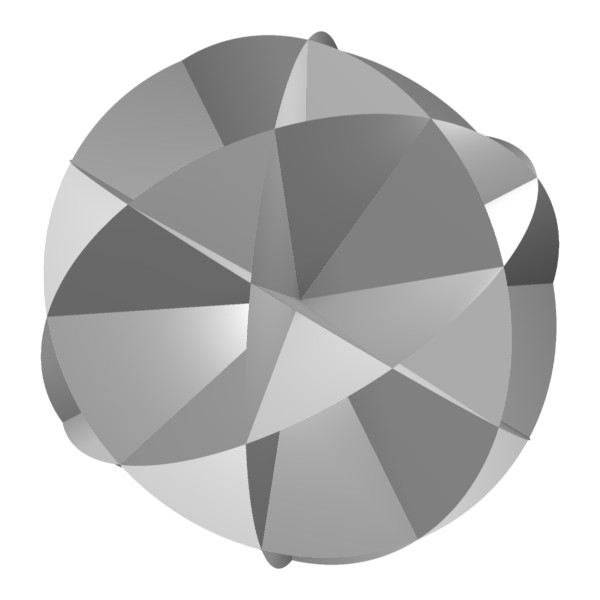
\includegraphics[width=1.4cm]{./../../common/images/barth_sextic_planes}
        \end{tabular}
        &
        \begin{tabular}{c@{}}
          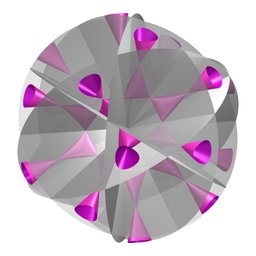
\includegraphics[width=1.4cm]{./../../common/images/barth_sextic_and_planes}
        \end{tabular}
      \end{tabular}
    \end{center}
    \vspace*{-0.1cm}

    The Barth Sextic satisfies the equation 
    $P_6 - \alpha K^2=0,$ where $P_6$
    denote the 
    six symmetry planes, $K=x^2+y^2+z^2-1$ is the unit sphere and 
    $\alpha=\frac{1}{4}(2+\sqrt{5})$.
\end{surferPage}
